% --------------------------------------------------------------
% Andrew Tindall
% --------------------------------------------------------------
 
\documentclass[12pt]{article}
 
\usepackage[margin=1in]{geometry} 
\usepackage{amsmath,amsthm,amssymb,enumitem, graphicx}
\setlist{
	listparindent=\parindent,
parsep=0pt,}

\newcommand{\N}{\mathbb{N}}
\newcommand{\Q}{\mathbb{Q}}
\newcommand{\Z}{\mathbb{Z}}
\newcommand{\R}{\mathbb{R}}
\newcommand{\mc}[1]{\mathcal{#1}}
\newcommand{\e}{\varepsilon}
\newcommand{\bs}{\backslash}
\newcommand{\PGL}{\text{PGL}}
\newcommand{\Sp}{\text{Sp}}
\newcommand{\tr}{\text{tr}}
\newcommand{\Lie}{\text{Lie}}
\newcommand{\rec}[1]{\frac{1}{#1}}
\newcommand{\toinf}{\rightarrow \infty}


\theoremstyle{definition}
\newtheorem{proofpart}{Part}
\newtheorem{theorem}{Theorem}
\makeatletter
\@addtoreset{proofpart}{theorem}
\makeatother


\newenvironment{problem}[2][Problem]{\begin{trivlist}
\item[\hskip \labelsep {\bfseries #1}\hskip \labelsep {\bfseries #2.}]}{\end{trivlist}}
 
\begin{document}
 
%\renewcommand{\qedsymbol}{\filledbox}
 
\title{Homework 2 }
\author{Andrew Tindall\\
	Analysis I}
 
\maketitle
\begin{problem}{1}
Let $s$ be the linear space of all sequences of real numbers.
\begin{enumerate}[label=(\roman*)]
    \item Prove that the function $d : s \times s \to \R$:
    \[
        d(\{x_i\}, \{y_i\}) := \sum_{i=1}^\infty \frac{1}{2^i}\frac{\lvert x_i - y_i \rvert}{1 + \lvert x_i - y_i\rvert}
    \] is a metric on $s$, and that the metric space $(s,d)$ is complete.
    
    \item Prove that every open neighborhood of $0$ in $s$ contains the whole line $\{\alpha x;\;\alpha \in \R\}$, for some $x \in s \bs \{0\}$.
    \item Deduce from (ii) that there is no norm in $s$, which would make it a Banach space, topologically equivalent to $(s,d)$.
\end{enumerate}
\end{problem}
\begin{proof}
	\begin{enumerate}[label=(\roman*)]
		\item	We show first that $d$ is well-defined and satisfies the axioms of a metric:
	\begin{itemize}
		\item $d$ is well-defined: Because each term in the series is bounded between $0 $ and $\frac{1}{2^i}$, and the series $\sum_{i=1}^\infty \frac{1}{2^i}$ converges to $1$, the series above must also exist, making $d$ a well-defined function.
		\item $d(x,y) \geq 0$: Because $d$ is defined as a series of nonnegative elements, it must be nonnegative.
		\item $d(x,y) = 0 \iff x = y$: The series will be zero if and only if each term is zero, which will occur only if $x_i = y_i$ for each component, which happens if and only if the two sequences are equal.
		\item $d(x,y) = d(y,x)$: The definition of $d$ is symmetric in $x_i$ and $y_i$, because $\left \lvert { x_i - y_i } \right \lvert  = \left \lvert { y_i - x_i } \right \lvert $.
		\item $d(x,z) \leq d(x,y) + d(y,z)$: We show that this inequality holds componentwise. Denote by $d'$ the metric on $\R$, $d'(x,y) = \left \lvert { x - y } \right \lvert $, and let $f$ be the function $f(x) = \frac{x}{1+x}$. Then $f' = \frac{1}{(1+x)^2}$, which is positive on $[0, \infty)$, so $f$ is a monotonic function on the nonnegative reals. In particular, since 
			\begin{align*}
				\left \lvert { x_i - z_i } \right \lvert \leq \left \lvert { x_i - y_i } \right \lvert  + \left \lvert { y_i - z_i } \right \lvert,
			\end{align*}
			We see that $f(\left \lvert { x_i - z_i } \right \lvert ) \leq f(\left \lvert { x_i - y_i } \right \lvert  + \left \lvert { y_i - z_i } \right \lvert )$. This shows that the triangle inequality holds:
			\begin{align*}
				\frac{\left \lvert { x_i - z_i } \right \lvert }{1 + \left \lvert { x_i - z_i } \right \lvert }
				&= f(d'(x,z))\\	
				&\leq f(d'(x,y) + d'(y,z))\\
			&= \frac{\left \lvert { x_i - y_i } \right \lvert + \left \lvert { y_i - z_i } \right \lvert}{1+ \left \lvert { x_i - y_i } \right \lvert + \left \lvert { y_i - z_i } \right \lvert }\\
			&= \frac{\left \lvert { x_i - y_i } \right \lvert }{1 + \left \lvert { x_i - y_i } \right \lvert  + \left \lvert { y_i - z_i } \right \lvert } + \frac{\left \lvert { y_i - z_i } \right \lvert }{ 1 + \left \lvert { x_i - y_i } \right \lvert + \left \lvert { y_i - z_i } \right \lvert }\\
			&\leq \frac{\left \lvert { x_i - y_i } \right \lvert }{1 + \left \lvert { x_i - y_i } \right \lvert } + \frac{\left \lvert { y_i - z_i } \right \lvert }{1 + \left \lvert { y_i - z_i } \right \lvert }
			\end{align*}
			Multiplying by a factor of $\frac{1}{2^i}$ and summing over $i$, we see that $d(x,z) \leq d(x,y) + d(y,z)$. Thus, the triangle inequality holds, and the function $d$ is a metric.
	\end{itemize}
	We now show that the space of sequences is complete under this metric. Let $\left\{ x^j \right\}$ be a sequence of sequences which is Cauchy under $d$; we show that there exists some sequence $x$ which the $x^j$s converge to.
	\par Fix an $i \in \N$ and $\varepsilon > 0$.  Because the sequence is cauchy, we may find an $N \in \N$ such that, for $j, k \geq N$, $d(x^j - x^k) < \frac{\varepsilon}{2^i}$. Then, because each term in the sum defining $d$ is bounded by the value of the sum itself, we see that
	\begin{align*}
		\frac{1}{2^i} \frac{\left \lvert { x^j_i - x^k_i } \right \lvert }{1 + \left \lvert { x^j_i - x^k_i } \right \lvert } \leq \sum_{i= 1}^\infty \\
		&= d(x^j,x^k)\\
		&< \frac{\varepsilon}{2^i}
	\end{align*}
	Thus the difference between the $i$th component of any two sequences $x^j, x^k$ is less than $\varepsilon$ for $j, k > \N$, and we get a cauchy sequence in each variable, which converges to a real number $x_i$ by the completeness of the reals. We can therefore construct a sequence $x$, where the $i$th component is equal to $x_i$. 
	\par We now show that the sequences $x^j$ converge to the sequence $x$ in the norm $d$. Let $\varepsilon > 0$, and let $k$ be such that $2^{k-1} < \epsilon$. For example, take $k := \left \lceil \log_2(1/\varepsilon) + 2 \right \rceil$. Then we can divide the norm $d(x^j, x)$ into two parts:
	\begin{align*}
		d(x^j, x) &= \sum_{i = 1}^\infty \frac{1}{2^i}\frac{\left \lvert { x^j_i - x_i } \right \lvert }{1 + \left \lvert { x^j_i - x_i } \right \lvert }\\
		&= \sum_{i = 1}^{k - 1} \frac{1}{2^i} \frac{\left \lvert { x^j_i - x_i } \right \lvert }{ 1 + \left \lvert { x^j_i - x_i } \right \lvert }+ \sum_{i = k}^\infty \frac{1}{2^i} \frac{\left \lvert { x^j_i - x_i } \right \lvert }{1 + \left \lvert { x^j_i - x_i } \right \lvert }
	\end{align*} 
	By the fact that each term is bounded by $\frac{1}{2^i}$, the sum on the right is less than or equal to $\sum_k^\infty \frac{1}{2^i} = \frac{1}{2^{k-1}}$, which by choice of $k$ is less than or equal to $\frac{\varepsilon}{2}$.
	\par The sum on the right is finite, and by the fact that the components $x^j_i$ converge to $x_i$, we may chose $k-1$ different $N_i$s, such that for $j \geq N_i$,
	\[ \frac{1}{2^i}\frac{\left \lvert { x^j_i - x_i } \right \lvert }{1 + \left \lvert { x^j - x_i } \right \lvert } < \frac{\varepsilon}{2(k-1)}.\]
	Therefore, combining our bounds for the sums on the left and the right,
	\begin{align*}
		d(x^j, x) &= \sum_{i = 1}^{k - 1} \frac{1}{2^i} \frac{\left \lvert { x^j_i - x_i } \right \lvert }{ 1 + \left \lvert { x^j_i - x_i } \right \lvert }+ \sum_{i = k}^\infty \frac{1}{2^i} \frac{\left \lvert { x^j_i - x_i } \right \lvert }{1 + \left \lvert { x^j_i - x_i } \right \lvert }\\
		&< \sum_{i=1}^{k-1} \frac{\varepsilon}{2(k-1)} + \sum_{i=k}^\infty 1\\
		&\leq \frac{\varepsilon}{2} + \frac{\varepsilon}{2} = \varepsilon
	\end{align*}
	Therefore, an arbitrary Cauchy sequence $x^j$ of sequences converges to a sequence $x$, and the space is complete.
\item Now, let $U$ be an open neighborhood of $0$ in the topology induced by the metric $d$. $U$ then contains some open ball of radius $\varepsilon$ around $0$. We can show that there exists a nonzero element $x$ such that the whole line $\left\{ \alpha x \mid \alpha \in \R \right\} $ is contained in this ball, and therefore in $U$.
	\par Let $k = \left \lceil \log_2 \varepsilon \right \rceil + 1$, and let $x$ be the vector defined by 
	\[x_i = \begin{cases}
			0 &i \leq k\\
			1 &k < i
\end{cases}\]
Then, for any $\alpha \in \R$, the distance between $x$ and $0$ is bounded by $\frac{\varepsilon}{2}$:
\begin{align*}
	d(\alpha x, 0) &= \sum_{i = 1}^\infty \frac{1}{2^i} \frac{\left \lvert { \alpha x_i } \right \lvert }{1 + \left \lvert { \alpha x_i } \right \lvert }\\
	&= \sum_{i=1}^{k-1} 0 + \sum_{i = k}^\infty \frac{\left \lvert { \alpha x_i  } \right \lvert }{1 + \alpha x_i}\\
	&\leq \sum_{i=k}^\infty \frac{1}{2^i}\\
	&\leq \frac{\varepsilon}{2}
\end{align*}
Thus, for any $\alpha$, $\alpha x$ is within the open ball $B_\varepsilon(0)$.
\item We may use this fact to show that there is no norm on $s$ which would make it a Banach space topologically equivalent to $(s,d)$. We use the definition that two topologies are equivalent if and only if their open sets are exactly the same. This is equivalent to the statement that every sequence which converges in one converges in the other, as the open sets in both normed and metric spaces may be defined by convergence of sequences, and convergence of sequences in any topological space may be defined in terms of open sets.
	\par Take some norm $\left \lVert { \cdot } \right \lVert $. If this norm made $s$ topologically equivalent to $(s,d)$, then every open set containing $0$ in $(s, \left \lVert { \cdot } \right \lVert )$ would contain an open set of $(s, d)$ that contained $0$, and in particular, the open unit ball $\left\{ x \in s \mid \left \lVert { x } \right \lVert < 1 \right\} $ would contain, by the fact that open balls form a basis, an open ball $B_\varepsilon(0)$ of vectors that are less than $\varepsilon$ away from $0$ in the metric $d$.
	\par As we have seen, any such open ball must contain the whole line $\left\{ \alpha x \mid \alpha \in \R \right\} $ for some vector $x$. Let $a = \left \lVert { x } \right \lVert $; then the vector $\frac{2}{a} x$ is also contained in this ball. However, by the axioms of a norm, $\left \lVert { \frac{2}{a} x } \right \lVert = \left \lvert { 2 } \right \lvert $, contradicting the assumption that $x$ is contained within the interior of the unit ball. Therefore, no norm can exist which makes $s$ topologically equivalent to $(s,d)$.
\end{enumerate}
\end{proof}
\begin{problem}{2}
	Prove that for every $x \neq y$ in a normed space $E$, then there exists some $T \in E^*$ such that $T(x) < T(y)$. 
\end{problem}
\begin{proof}
	There are two possibilities: either $y = ax$ for some $a \in \R$, or $x$ and $y$ are linearly independent.
	\begin{itemize}
		\item If $x = ay$, then the space $E_0$ spanned by $x$ and $y$ is a one dimensional linear subspace of $E$, and the set $\left\{ y \right\}$ is a Hamel basis of $E_0$. There are two possibilities here: either $a < 1$ or $a > 1$. 
			\par If $a < 1$, then let $T_0 : E_0 \to \R$ be defined by extending the function $y \mapsto 1$. Then \begin{align*}
				T_0(x) &= T_0(ay)\\
				&= aT_0(y)\\
				&= a\\
				&< 1\\
				&= T_0(y)
			\end{align*}
			\par On the other hand, if $a > 1$, then let $T_0$ be defined by extending the function $y \mapsto -1$. Then
			\begin{align*}
				T_0(x) &= T_0(ay)\\
			&= aT_0(y)\\
			&= -a\\
			&< -1\\
		&= T_0(y)
			\end{align*}
		\item If $x$ and $y$ are linearly independent, then the set $\left\{ x,y \right\}$ forms a Hamel basis for the space spanned by $x$ and $y$, and we may define a linear functional by extending the map sending $x \mapsto -1$ and $y \mapsto 1$.
	\end{itemize}
	So in the three cases, we have found a subspace $E_0$ of $E$ containing $x$ and $y$, and a linear functional $T_0$ for which $T_0(x) < T_0(y)$. By exercise $5$ of the last homework, there exists a linear functional $T$ from $E \to \R$ which agrees with $T_0$ on $E_0$, and so $T(x) < T(y)$.
\end{proof}
\begin{problem}{3}
	Find the norms of the following linear functionals on $\mathcal{C}[a,b]$, with the norm of the uniform convergence $\left \lVert { f } \right \lVert  = \max\left\{ \left \lvert { f(x) } \right \lvert ; x \in [a,b] \right\}$.
	\begin{enumerate}[label=(\roman*)]
		\item $T(f) := \int_a^b f(x)d(x)$
		\item $T_g(f) := \int_a^bf(x)g(x)dx$, where $g$ is some fixed element of $\mathcal{C}[a,b]$.
		\item $T(f) := \sum_{i=1}^n \lambda_i \cdot f(x_i)$, where $x_1\dots x_n \in [a,b]$ and $\lambda_1 \dots \lambda_n \in \R$ are given parameters.
	\end{enumerate}
\end{problem}
\begin{proof}
		In the following, let $A = b-a$.
	\begin{enumerate}[label=(\roman*)]
		\item It is quick to see that $\left \lVert { T } \right \lVert  = A$, and that this maximum is attained for the functions $f_1(x) = 1$ and $f_2(x) = -1$. This follows from the fact (found in \cite{rudin}) that, on a measurable space $\Omega$ with $\mu(\Omega) = 1$, 
			\[\inf\left\{ f(x); x \in \Omega \right\} \leq \int_\Omega f(x) \leq \sup\left\{ f(x); x \in \Omega \right\}\]
			In particular, with $\Omega = [a,b]$ and $\mu(X) = m(X)/A$, where $m$ is the standard Lesbesge measure on $\R$, this shows
			\[\min\left\{ f(x); a \leq x \leq b \right\} \leq \frac{1}{A} \int_a^b f(x) dx \leq \max\left\{ f(x); a \leq x \leq b \right\}\]
			In particular, if $\left \lVert { f } \right \lVert  = 1$, then 
			\[ -1 \leq \frac{1}{A}\int_a^b f(x)dx \leq 1\]
			So the norm of $T$ is bounded by $A$. It reaches this value for the constant function taking $x \mapsto 1$, as $\int_a^b 1 dx = (a-b) = A$.

		\item Fix some function $g \in \mathcal{C}[a,b]$. Let $g_+$ and $g_-$ be the positive and negative parts of $g$, defined by 
			\begin{align*}g_+(x) &= \begin{cases}
					g(x) & g(x) > 0\\
					0 & g(x) \leq 0
			\end{cases}\\
		g_-(x) &= g_+(x) - g(x)  \end{align*}
		In particular, these functions are measurable under the Lesbesgue measure, since $g_+$ is the pointwise maximum of two measurable functions,  $g$ and the constant function $0$. We will see that the norm of $T_g$ is equal to 
		\[\int_a^b g_+(x) dx - \int_a^b g_-(x) dx\]
		We first bound the value of $\left \lVert { T_g } \right \lVert $ by this value. Let $f \in \mathcal{C}[a,b]$ have norm $\left \lVert { f } \right \lVert = 1$. Then 
		\begin{align*}
			T_g(f) &= \int_a^b f(x)g(x)dx\\
			&= \int_a^b f(x) (g_+(x) + g_-(x)) dx\\
			&= \int_a^b f(x)g_+(x)dx + \int_a^b f(x)g_-(x)dx
		\end{align*}
		Since $-1 \leq f(x) \leq 1$ on the interval $[a,b]$, and $g_+(x)$ is nonnegative, the value of $\int_a^bf(x)g_+(x) dx$ is bounded by 
		\begin{equation} -\int_a^b g_+(x)dx  \leq \int_a^b f(x)g_+(x) dx \leq \int_a^b g(x)dx \label{pos}\end{equation}
		\par Similarly, because $g_-(x) \leq 0$ on $[a,b]$, the value of $\int_a^b f(x)g_-(x)dx$ is bounded by
		\begin{equation} \int_a^b g_-(x)dx \leq \int_a^b f(x)g_-(x)dx \leq -\int_a^b g_-(x)dx\label{neg}\end{equation}
		If the leftmost inequalities in \ref{pos} and \ref{neg} are satisfied, then 
		\[ T_g(f) = -\left( \int_a^b g_+(x)dx - \int_a^b g_-(x)dx \right).\]
		And if the rightmost inequalities are satisfied, then
		\[ T_g(x) = \int_a^b g_+(x)dx + \int_a^b g_-(x)dx.\]
		In either case, we see that $\left \lvert { T(f) } \right \lvert = \int_a^b g_+(x)dx + \int_a^b g_-(x)dx$, and that in any other case, $\left \lvert { T(f) } \right \lvert < \int_a^b g_+(x)dx + \int_a^b g_-(x)dx$. Thus the norm is bounded by this value.
		\par In fact, we can show that it is always exactly this value, although it may not be that the value is attained anywhere on the unit sphere. Let $P = g^{-1}(\left[ 0, \infty \right))$ be the set of points where $g$ is nonnegative, and $N = g^{-1}( (-\infty, 0))$ be the set where $g$ is negative. 
		\par Let $\chi_P$ and $\chi_N$ be the characteristic functions of these (measurable) sets. Then the function $\chi_P - \chi_N$ is a measurable function, and we may approximate it with a sequence of continuous functions $\left\{ f_n \right\}$ of norm $1$ - this is easy to see if the sets $P$ and $N$ are well-behaved, such as if they are finite unions of intervals, but a little trickier in the infinite case - I do think it is always true, however.
		\par Once we have such a sequence of bounded continuous functions $f_n$ of norm $1$, which converge to the measurable function $\chi_P - \chi_N$, we see from a theorem in \cite{rudin} that the integrals of these functions converge:
		\begin{align*}
			\lim_{n\to \infty}\left \lvert { T_g(f_n) } \right \lvert &= \lim_{n\to \infty}\left \lvert\int_a^b f_n(x)g(x)dx\right \rvert\\
			&= \left \lvert\int_a^b (\lim_{n\to\infty}f_n(x))g(x)dx\right \rvert\\
			&= \left \lvert\int_a^b (\chi_P - \chi_N)g(x)dx\right \rvert\\
			&= \left \lvert \int_P g(x) - \int_N g(x)\right\rvert\\
			&= \left \lvert { \int_a^b g_+(x)dx - \int_a^b g_-(x)dx } \right \lvert 
		\end{align*}
		So the supremum for $\left \lvert { T_g(f) } \right \lvert $ on the unit sphere is indeed $\int_a^b g_+(x)dx - \int_a^b g_-(x)dx$, and therefore this is the norm of $T_g$.
	\item We show that the norm of $T$ is $\sum_{i=1}^n \left \lvert { \lambda_i } \right \lvert $, assuming that the given points $x_i$ are distinct - if they are not, we only need to do a little modification of the parameters $ \lambda_i$ to attain a $T'$ that is equal, and defined using distinct points $x_i$. 
	\par If, first of all, there exist a pair of points $x_j, x_k$, such that $x_j = x_k$, then define a new operator $T'$ by $\left (\sum_{i \neq j, k}^n \lambda_i \cdot f(x_i) \right )+ (\lambda_j + \lambda_k) \cdot f(x_j)$. By repeating this operation if necessary, we find an operator $T$ which is equal to the original, but defined only using distinct points $x_i$.
	\par Now, because $\left \lvert { f(x) } \right \lvert \leq 1$ for each $f$ in the unit sphere, we see that the value of $\left \lvert { T(f) } \right \lvert $ is bounded by 
	\[ \left \lvert { T(f) } \right \lvert \leq  { \sum_{i=1}^n } \left \lvert \lambda_i \right \lvert \]
	We now show that this is in fact the supremum of $T(f)$ for $\left \lVert { f } \right \lVert = 1$. For each $1 \leq i \leq n$, take the point $x_i$ and parameter $\lambda_i$, and define the point $p_i = (x_i, 1)$ if $\lambda_i > 0$, and $p_i = (x_i, -1)$ if $\lambda_i \leq 0$. It is not hard to construct a function which has norm $1$ and passes through these points - assume (perhaps by reordering) that the points are ordered, $x_1 < x_2 < \dots x_n$, and make a function such as the one pictured in Figure \ref{fig:function}. 
	\begin{figure}
		\centering
		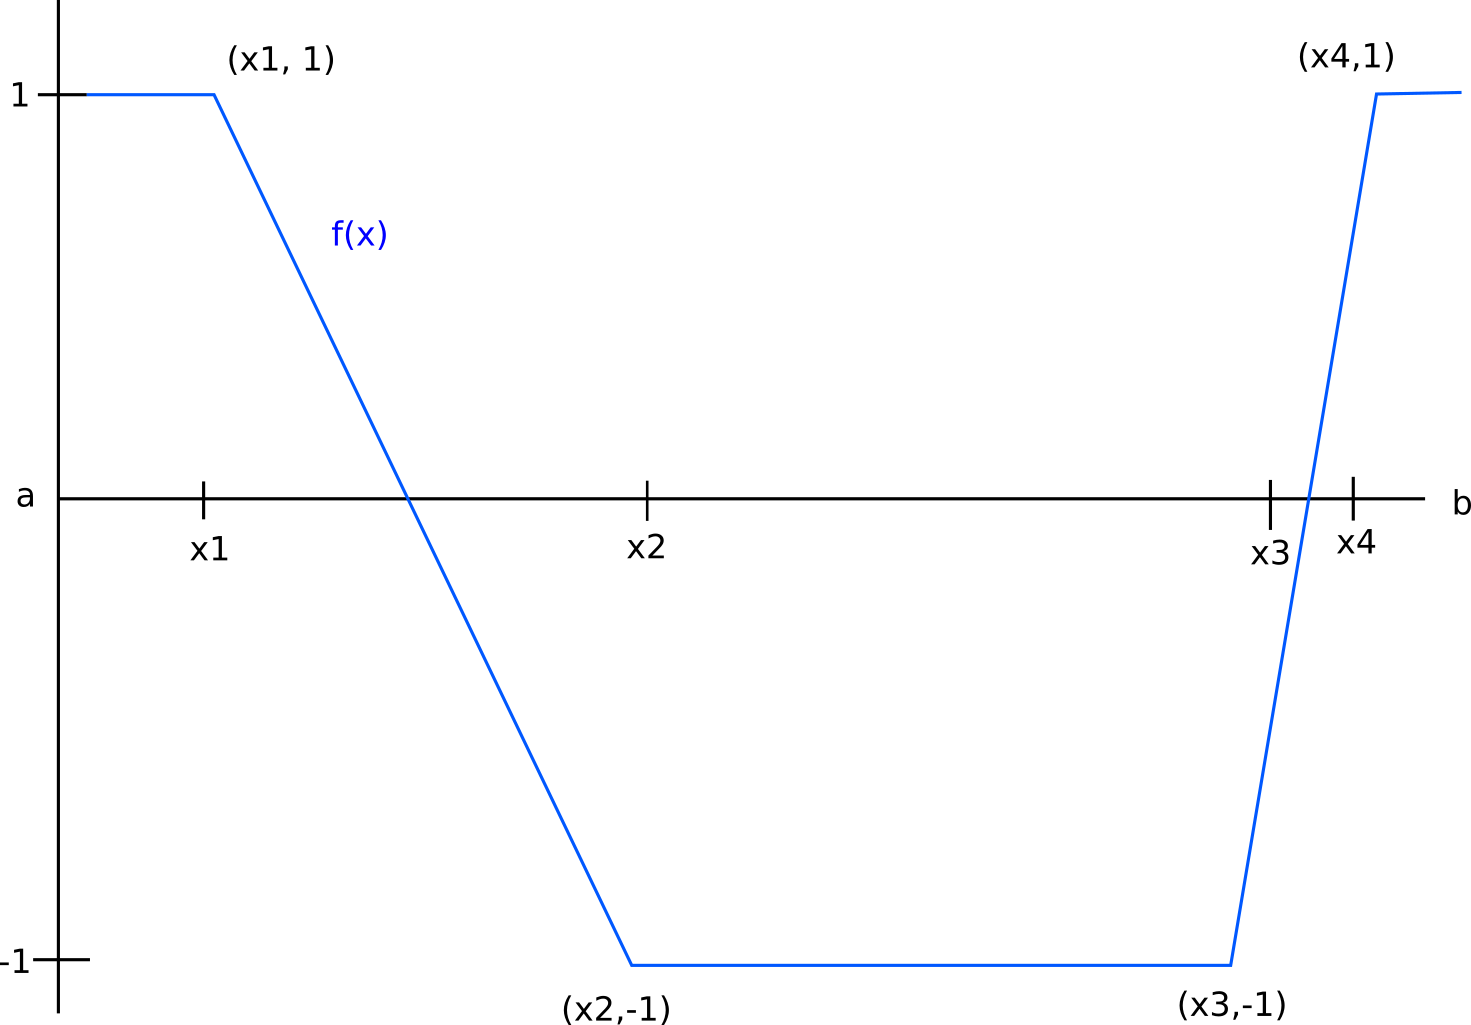
\includegraphics{hw_2_function.png}
		\caption{A continuous function which maximizes $\left \lvert { T(f) } \right \lvert $}
		\label{fig:function}
	\end{figure}
	In this case, the first point is greater than $a$, the signs of the four parameters $\lambda_i$ are $1, -1, -1, 1$, and the last point is less than $b$. Slight modifications would need to be made if, say, $x_1 = a$ and $\lambda_1 < 0$, in which case $f(a) = -1$ instead of $1$. But this is essentially a simple function to construct, and is always continuous.
	\par Because $f(x_i) = \text{sgn}(\lambda_i)$, we see that 
	\begin{align*}\left \lvert { T(f) } \right \lvert  &= \left \lvert { \sum_{i=1}^n } \lambda_i \text{sgn}(\lambda_i)\right \lvert \\
	&= \sum_{i=1}^n \left \lvert { \lambda_i } \right \lvert \end{align*}
	Therefore the supremum of $\left \lvert { T(f) } \right \lvert $ over $\left \lVert { f } \right \lVert  = 1$ is $\sum_{i=1}^n \left \lvert { \lambda_i } \right \lvert $.
	\end{enumerate}
\end{proof}
\begin{problem}{4}
	A normed space $E$ is ``strictly convex'' if and only if, for all $x \neq y \in E$, and for all $t \in (0,1)$, if $\left \lVert { x } \right \lVert  = \left \lVert { y } \right \lVert  = 1$ then $\left \lVert { tx + (1-t)t } \right \lVert < 1$.
	\par Prove that if $E^*$ is strictly convex then, for every $x_0 \in E$ there exists exactly one function $T \in E^*$ such that $\left \lVert { T } \right \lVert = \left \lVert { x_0 } \right \lVert $ and $T(x_0) = \left \lVert { x_0 } \right \lVert^2$.
\end{problem}
\begin{proof}
	We see first that the functions $T \in E^*$ with norm $\left \lVert { T } \right \lVert  = 1$ and $T(x_0) = \left \lVert { x_0 } \right \lVert ^2$ are, by scaling by a factor of $\frac{1}{\left \lVert { x_0 } \right \lVert }$, in a one-to-one correspondence with functions $T' \in E^*$ with norm $ 1  $ that take $T'(x_0) = \left \lVert { x_0 } \right \lVert $. So we show that there exists exactly one linear functional $T'$ with these properties.
	\par There certainly exists one such functional. The following existence proof is adapted from one in \cite{bachman}. Consider first the subspace $E_0$ of $E$ consisting of all scalar multiples of $x_0$. The functional $T_0$ defined by extending the map $x_0 \mapsto \left \lVert {  x_0 } \right \lVert $, taking any vector $\alpha x_0 \mapsto \alpha\left \lVert { x } \right \lVert $, is a well-defined linear functional on the space $E_0$.
	\par Further, this functional is bounded, as there are only two vectors in $E_0$ with norm $1$, and the value of $\left \lvert { T_0 } \right \lvert $ on each one is $1$. Therefore there is a convex symmetric functional which bounds $\lvert T_0(x) \rvert$ - specifically, the symmetric functional $p(x) = \left \lVert { x } \right \lVert $ - and therefore, by the Hahn-Banach theorem, we may extend the linear functional $T_0$ to a linear functional $T$ on the whole space $E$, such that $T\rvert_{E_0} = T_0$, and  $\lvert T(x) \rvert \leq p(x) = \left \lVert { x } \right \lVert $ for all $x \in E$. 
	\par This implies that the norm of $T$ is at most $1$, because for any $x$ such that $\left \lVert {  x } \right \lVert  = 1$, 
	\[ \left \lvert { T(x) } \right \lvert  \leq \left \lVert { x } \right \lVert  = 1.\]
	In fact, $\left \lVert { T } \right \lVert $ is equal to $1$, because $T(\frac{x_0}{\left \lVert { x_0 } \right \lVert }) = 1$, and $\left \lVert { \frac{x_0}{\left \lVert { x_0 } \right \lVert } } \right \lVert  = 1$. So this linear functional takes $x_0$ to $\left \lVert { x_0 } \right \lVert $, and its norm is exactly $1$.
	\par On the other hand, we may show that this is the only linear functional with these properties. Let $S$ and $T$ be two distinct linear functionals with norm $1$ which take $x_0$ to $\left \lVert { x_0 } \right \lVert $. Then, by strict convexity, we know that
	\begin{align*}
		\left \lVert { \frac{1}{2} S + \frac{1}{2} T } \right \lVert &< \frac{1}{2} \left \lVert { S } \right \lVert + \frac{1}{2} \left \lVert { T } \right \lVert\\
		&= \frac{1}{2} + \frac{1}{2} = 1
	\end{align*}
	However, the functional $\frac{1}{2}S + \frac{1}{2} T$ takes the unit vector $\frac{x_0}{\left \lVert { x_0 } \right \lVert }$ to the value $\frac{1}{2} \frac{\left \lVert { x_0 } \right \lVert }{\left \lVert { x_0 } \right \lVert } + \frac{1}{2}\frac{\left \lVert { x_0 } \right \lVert }{\left \lVert { x_0 } \right \lVert } = 1$, so the norm of $\frac{1}{2}S + \frac{1}{2} T$ must be at least $1$, a contradiction. Thus there must be at most one functional with the given properties. We see therefore that there is exactly one such functional.
\end{proof}
\begin{problem}{5}
	In the linear space $c_0$ of all real sequences converging to $0$, consider the sequence $\left\{ e^i \right\}_{i=1}^\infty$, where $e^i = \left( 0,0,0,\dots,1,0,\dots \right)$ with a $1$ in the $i$th place and $0$s in everywhere else.
	\begin{enumerate}[label=(\roman*)]
		\item Prove that $\left\{ e^i \right\}_{i=1}^\infty$ is a Schauder basis in $l_2$.
		\item Prove that $\left\{ e^i \right\}_{i=1}^\infty$ is a Schauder basis in $c_0$, normed by $l_\infty$.
	\end{enumerate}
\end{problem}
\begin{proof}
	\begin{enumerate}[label=(\roman*)]
		\item  We first show that $\left\{ e^i \right\}_{i=1}^\infty$ is a Schauder basis in the space $l_2$, with the $l_2$ norm. Fix $x \in l_2$; we first show that there is at least $1$ sequence $\left\{ \alpha_i \right\}$ of scalars in $\R$ such that 
			\[ x = \sum_{i=1}^\infty \alpha_i e^i.\]
		We will then show that this sequence is unique.
		\par The convergence of this sum is understood with respect to the topology induced by $l_2$ - that is, 
		\[\lim_{n\to\infty}  \left \lVert x -  \sum_{i=1}^n \alpha_i e^i \right \rVert_2 = 0\]
		\par We define the sequence $\alpha_i$ to be the same sequence as $x$ - that is, $\alpha_i = x_i$. Denote by $\left\{ x_i \right\}_{i=1}^n$ the sequence $x_1, \dots, x_n, 0, \dots$ which has its first $n$ elements equal to $x$'s, and then zeroes. Then we may calculate the limit above:
		\begin{align*}
			\lim_{n\to \infty} \left \lVert { x - \sum_{i=1}^n \alpha_i e^i } \right \lVert &= \lim_{n \to \infty}\left \lVert { \left\{ x_i \right\}_{i=1}^\infty - \left\{ x_i \right\}_{i=1}^n } \right \lVert \\
			&= \lim_{n\to \infty} \left \lVert \left\{ {x_i }\right\}_{i=n+1}^\infty  \right \lVert \\
			&= \lim_{n\to \infty} \left( \sum_{i=n+1}^\infty \left \lvert { x_i } \right \lvert ^2\right)^{1/2}
		\end{align*}
		Because $\left\{ x_i \right\}$ is in $l_2$, we know that the series $\sum_{i=1}^\infty \left \lvert { x_i } \right \lvert^2$ must converge to $\left \lVert { x } \right \lVert ^2$, and the converge of this series implies that the $n+1$-tails of the series converge to zero as $n$ goes to $0$. Therefore the limit above exists, and is equal to zero:
		\begin{align*}
		\lim_{n \to \infty} \left( \sum_{i=n+1}^\infty \left \lvert { x_i } \right \lvert ^2 \right)^{1/2} = \left( \lim_{n\to\infty} \sum_{i=n+1}^\infty \left \lvert { x_i } \right \lvert ^2 \right)^{1/2} = 0
		\end{align*}
		Thus there exists \textit{a} sequence of coefficients $\alpha_i$ such that $\sum_{i=1}^\infty \alpha_i e^i$ converges to $x$. We now show that this sequence is unique.
		\par If it were not, there would be a distinct sequence of coefficients $\alpha'$ which differed from $\alpha$ in at least one position, say in the $j$th. But then this $\alpha'_j \neq x_j$, and the norms of the differences between the sequences would not go to zero. Taking $n > j$ in the following calculation:
		\begin{align*}
			\lim_{n\to \infty} \left \lVert { x - \sum_{i=1}^n \alpha'_i e^j } \right \rVert &= \lim_{n\to \infty} \left( \sum_{i=1}^n \left \lvert { x_i - \alpha'_i } \right \lvert ^2 + \sum_{i=n+1}^\infty \left \lvert { x_i } \right \lvert ^2 \right)^{1/2}	\\
			&\geq \left( \sum_{i=1}^n \left \lvert { x_i - \alpha'_i } \right \lvert ^2  \right)^{1/2}\\
			&\geq \left( \left \lvert { x_j - \alpha'_j } \right \lvert ^2 \right)^{1/2}\\
			&= \left \lvert { x_j - \alpha'_j } \right \lvert \\
			&> 0.
		\end{align*}
		Therefore there is exactly one sequence of coefficients $\alpha_i$ for which $x = \sum_{i=1}^\infty \alpha_ie^i$.
	\item We now show that $e^i$ is also a Schauder basis for the space $c_0$ with the $l_\infty $ norm. Let $x$ be an arbitrary convergent sequence in $c_0$, and let $\alpha_i = x_i$ once again be defined by letting the coefficients $\alpha_i$ be the same as the elements in the sequence $x$. We show first that 
		\[ \lim_{n\to \infty} \left \lVert { x - \sum_{i=1}^n \alpha_i e^i } \right \lVert = 0.\]
Again, we may change the term inside the norm to be simply the tail of the sequence $x$ (considered as a sequence where the first $n$ terms are simply $0$):
		\begin{align*}
		\lim_{n\to \infty} \left \lVert { x - \sum_{i=1}^n \alpha_i e^i } \right \lVert &= \lim_{n\to \infty} \left \lVert { \left\{ x_i \right\}_{i=n+1}^\infty } \right \lVert \\
		&= \lim_{n\to\infty}\sup_{i \geq n+1} \left \lvert { x_i } \right \lvert 
	\end{align*}
	The convergence of the sequence $\{x_i\}$ to $0$ says exactly that the above limit exists and is equal to zero. Thus, $x = \sum_{i=1}^\infty \alpha_i e^i$.
	\par We can now show that this is the only sequence of coefficients $\alpha_i$ with this property. Let $\alpha'_i$ be some other set of coefficients which differs from $x$ in at least one spot; say that $\lvert \alpha'_j - x_j\rvert > 0 $ for some $j$. Then (assuming between lines $2$ and $3$ that $n > j$):
	\begin{align*}
		\lim_{n \to \infty}\left \lVert { x - \sum_{i=1}^n \alpha'_i e^i } \right \lVert  &= \lim_{n \to \infty} \sup_{i \geq 1} \left \lvert { \left (x - \sum_{i=1}^n \alpha'_i e^i   \right )_i} \right \rvert \\
		&\geq \lim_{n\to \infty} \left \lvert \left( x - \sum_{i=1}^n \alpha'_i e^j\right)_j\right \rvert\\
	&= \lim_{n \to \infty} \left \lvert { x_j - \alpha'_j } \right \lvert \\
	&> 0
	\end{align*}
	Therefore there is exactly one set of coefficients $\alpha_i$ such that $x = \sum_{i=1}^\infty \alpha_i e^i$, and the set is a Schauder basis.	
	\end{enumerate}
\end{proof}
\begin{thebibliography}{}
	\bibitem{rudin}{Rudin, W. Real and Complex Analysis, 3rd Edition. McGraw Hill, 1986.} 
	\bibitem{bachman}{Bachman, G. and Narici, L. Functional Analysis. Dover, 2000. (Original work published 1966.) }
\end{thebibliography}

\end{document}
